Closed-loop simulations with the control logic of the zigzag test were used to predict the model test experiments. Comparisons of these predictions are shown in \autoref{fig:closed_loop_zigzag10} and \autoref{fig:closed_loop_zigzag20}. The drift angle $\beta$, heading angle $\psi$, and yaw rate $r$ are in good agreement with the experiments for all the models, especially the heading, which is the most critical in zigzag tests. However, the PU model exhibits a faster response time.

\begin{figure}
    \centering
    \begin{subfigure}[b]{0.49\textwidth}
        \centering
        \includesvg[width=\columnwidth]{figures/results.closed_loop_zigzag10.svg}
        \caption{zigzag10/10.}
        \label{fig:closed_loop_zigzag10}
    \end{subfigure}
    \hfill
    \begin{subfigure}[b]{0.49\textwidth}
        \centering
        \includesvg[width=\columnwidth]{figures/results.closed_loop_zigzag20.svg}
        \caption{zigzag20/20.}
        \label{fig:closed_loop_zigzag20}
    \end{subfigure}
    \caption{Closed-loop simulations compared with model test.}
    \label{fig:closed_loop}
\end{figure}
%\begin{figure}[h]
%    \centering
%    \includesvg[width=\columnwidth]{figures/results.closed_loop_zigzag10.svg}
%    \caption{Results from a zigzag10/10 model test compared with closed loop simulations.}
%    \label{fig:closed_loop_zigzag10}
%\end{figure}
%\begin{figure}[h]
%    \centering
%    \includesvg[width=\columnwidth]{figures/results.closed_loop_zigzag20.svg}
%    \caption{Results from a zigzag20/20 model test compared with closed loop simulations.}
%    \label{fig:closed_loop_zigzag20}
%\end{figure}
ID comparisons are shown in \autoref{fig:ID_zigzag10} for the zigzag10/10 and in \autoref{fig:ID_zigzag20} for the zigzag20/20, providing more detailed information about the forces and moments involved during the manoeuvres. The models predict the forces and moments for the estimated state of the experiment. Thus, all models predict the same state in contrast to simulations, where the states may differ as the solutions begin to deviate.    
The total yawing moments $N_D$ agree well for all models and the experimental data. For the total sway force $Y_R$, the PU model predicts a slightly higher force.  

Furthermore, the reference and PI models predict the same rudder yawing moment $N_R$ since they use the same deterministic semi-empirical rudder model; the yawing moments from the hull $N_H$ are, therefore, also similar for these models. On the other hand, the rudder yawing moment from the PU model is very different. The regression has thus also yielded very different yawing moments from the hull $N_H$ so that the total yawing moment is correct. 
While the total yawing moment is the same for all models, the decomposition of hull and rudder moments vary significantly. Erroneous decomposition is not a major problem as long as all of the components are active, but if one disappears---e.g., when the rudder angle is small---large errors appear from the remaining components, and the model generalization deteriorates.  
\begin{figure}[h]
    \centering
    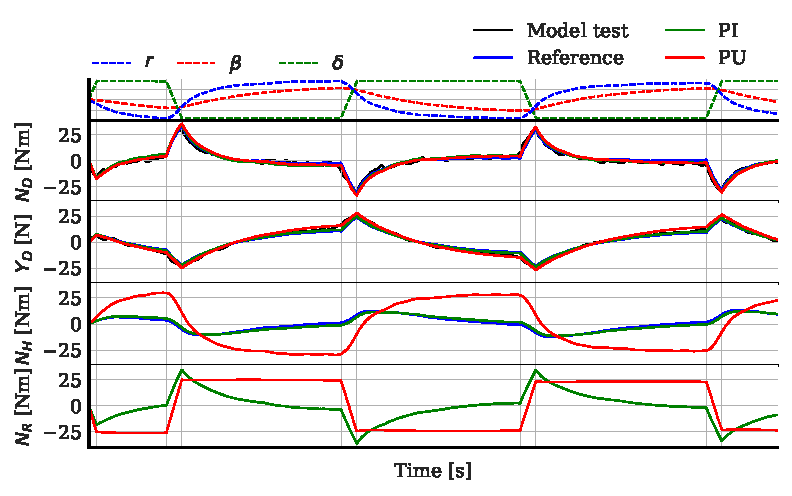
\includegraphics{figures/results.ID_zigzag10.pdf}
    \caption{ID estimations of $Y_D$ and $N_D$ during a zigzag10/10 model test compared with model predictions.}
    \label{fig:ID_zigzag10}
\end{figure}
\begin{figure}[h]
    \centering
    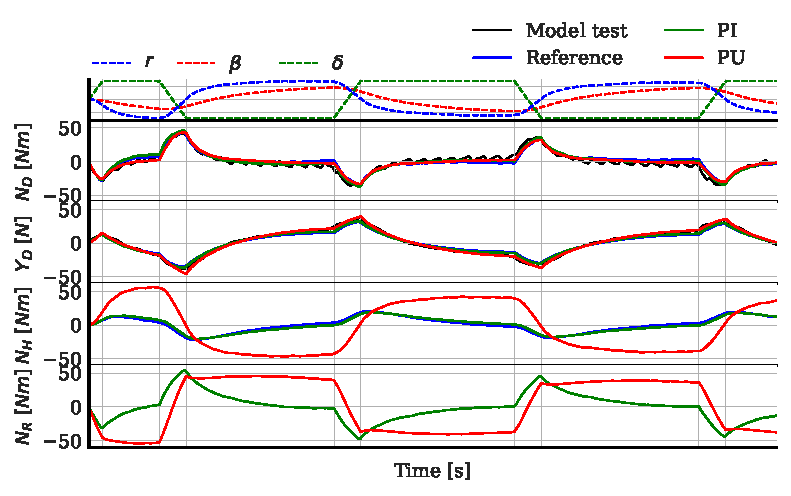
\includegraphics{figures/results.ID_zigzag20.pdf}
    \caption{ID estimations of $Y_D$ and $N_D$ during a zigzag20/20 model test compared with model predictions.}
    \label{fig:ID_zigzag20}
\end{figure}
\FloatBarrier

The hull force model can be closely examined by decomposing the individual parameter contributions. \autoref{fig:ID_regression_N_decomposition} shows the parameter decomposition for the two models and the reference model, indicating the combined contributions for drift and yaw rate parameters. The PI  and reference models have very similar parameter decompositions.
However, the parameter decomposition of the PU model is completely different, where almost the entire contribution to the hull yawing moment $N_H$ can be ascribed to the yaw rate parameters. The sway force due to drift is also considerable.  
\begin{figure}[h]
    \begin{center}
        \includesvg{figures/results.hull_force_decomposition_zigzag20.svg}
        \caption{Decomposition of hull forces and moments during a zigzag20/20 test for parameters related to drift, yaw rate the prediction models.}
        \label{fig:ID_regression_N_decomposition}
    \end{center}
\end{figure}
The following section further investigates the possible implications of this physically incorrect decomposition.